\documentclass[11pt,a4paper,titlepage,svgnames]{article}
\usepackage[a4paper]{geometry}
\usepackage[utf8]{inputenc}
\usepackage[german]{babel}
\usepackage{lipsum}
\usepackage{tikz}
\usetikzlibrary{arrows.meta}
\usepackage{tikz-uml}

\usepackage{amsmath, amssymb, amsfonts, amsthm, fouriernc, mathtools}
% mathtools for: Aboxed (put box on last equation in align envirenment)
\usepackage{microtype} %improves the spacing between words and letters

\usepackage{tabularx}
\usepackage{graphicx}
\graphicspath{ {./pics/} {./eps/}}
\usepackage{epsfig}
\usepackage{epstopdf}
\usepackage{listings}
\usepackage[numbered,framed]{matlab-prettifier}
\lstset{literate=%
	{Ö}{{\"O}}1
	{Ä}{{\"A}}1
	{Ü}{{\"U}}1
	{ß}{{\ss}}1
	{ü}{{\"u}}1
	{ä}{{\"a}}1
	{ö}{{\"o}}1
}

\usepackage{csquotes}
\MakeOuterQuote{"}

%%%%%%%%%%%%%%%%%%%%%%%%%%%%%%%%%%%%%%%%%%%%%%%%%%
%% COLOR DEFINITIONS
%%%%%%%%%%%%%%%%%%%%%%%%%%%%%%%%%%%%%%%%%%%%%%%%%%
\usepackage[]{xcolor} % Enabling mixing colors and color's call by 'svgnames'
%%%%%%%%%%%%%%%%%%%%%%%%%%%%%%%%%%%%%%%%%%%%%%%%%%
\definecolor{MyColor1}{rgb}{0.2,0.4,0.6} %mix personal color
\newcommand{\textb}{\color{Black} \usefont{OT1}{lmss}{m}{n}}
\newcommand{\blue}{\color{MyColor1} \usefont{OT1}{lmss}{m}{n}}
\newcommand{\blueb}{\color{MyColor1} \usefont{OT1}{lmss}{b}{n}}
\newcommand{\red}{\color{LightCoral} \usefont{OT1}{lmss}{m}{n}}
\newcommand{\green}{\color{Turquoise} \usefont{OT1}{lmss}{m}{n}}
%%%%%%%%%%%%%%%%%%%%%%%%%%%%%%%%%%%%%%%%%%%%%%%%%%

\lstdefinestyle{customc++}{
	belowcaptionskip=1\baselineskip,
%	breaklines=true,
	frame=tb,
	tabsize=2,
%	xleftmargin=\parindent,
	language=C++,
	showstringspaces=false,
	basicstyle=\footnotesize\ttfamily,
	keywordstyle=\bfseries\color{blue},
	commentstyle=\itshape\color{orange},
	identifierstyle=\color{black},
	stringstyle=\color{orange},
	backgroundcolor=\color{black!5},
}
\lstset{style=customc++ }



%%%%%%%%%%%%%%%%%%%%%%%%%%%%%%%%%%%%%%%%%%%%%%%%%%
%% FONTS AND COLORS
%%%%%%%%%%%%%%%%%%%%%%%%%%%%%%%%%%%%%%%%%%%%%%%%%%
%    SECTIONS
%%%%%%%%%%%%%%%%%%%%%%%%%%%%%%%%%%%%%%%%%%%%%%%%%%
\usepackage{titlesec}
\usepackage{sectsty}
%%%%%%%%%%%%%%%%%%%%%%%%
%set section/subsections HEADINGS font and color
\sectionfont{\color{MyColor1}}  % sets colour of sections
\subsectionfont{\color{MyColor1}}  % sets colour of sections
\subsubsectionfont{\color{MyColor1}}  % sets colour of sections

%set section enumerator to arabic number (see footnotes markings alternatives)
\renewcommand\thesection{\arabic{section}.} %define sections numbering
\renewcommand\thesubsection{\thesection\arabic{subsection}} %subsec.num.

%define new section style
\newcommand{\mysection}{
	\titleformat{\section} [runin] {\usefont{OT1}{lmss}{b}{n}\color{MyColor1}} 
	{\thesection} {3pt} {} } 

%%%%%%%%%%%%%%%%%%%%%%%%%%%%%%%%%%%%%%%%%%%%%%%%%%
%		CAPTIONS
%%%%%%%%%%%%%%%%%%%%%%%%%%%%%%%%%%%%%%%%%%%%%%%%%%
\usepackage{caption}
\usepackage{subcaption}
%%%%%%%%%%%%%%%%%%%%%%%%
\captionsetup[figure]{labelfont={color=Black}}

%%%%%%%%%%%%%%%%%%%%%%%%%%%%%%%%%%%%%%%%%%%%%%%%%%
%		!!!EQUATION (ARRAY) --> USING ALIGN INSTEAD
%%%%%%%%%%%%%%%%%%%%%%%%%%%%%%%%%%%%%%%%%%%%%%%%%%
%using amsmath package to redefine eq. numeration (1.1, 1.2, ...) 
%%%%%%%%%%%%%%%%%%%%%%%%
\renewcommand{\theequation}{\thesection\arabic{equation}}

%set box background to grey in align environment 
\usepackage{etoolbox}% http://ctan.org/pkg/etoolbox
\makeatletter
\patchcmd{\@Aboxed}{\boxed{#1#2}}{\colorbox{black!15}{$#1#2$}}{}{}%
\patchcmd{\@boxed}{\boxed{#1#2}}{\colorbox{black!15}{$#1#2$}}{}{}%
\makeatother
%%%%%%%%%%%%%%%%%%%%%%%%%%%%%%%%%%%%%%%%%%%%%%%%%%

% make the font in the toc 
\newcommand{\argmin}{\mathop{\mathrm{argmin}}}

%\makeatletter
%\let\reftagform@=\tagform@
%\def\tagform@#1{\maketag@@@{(\ignorespaces\textcolor{red}{#1}\unskip\@@italiccorr)}}
%\renewcommand{\eqref}[1]{\textup{\reftagform@{\ref{#1}}}}
%\makeatother
\usepackage{hyperref}
\hypersetup{colorlinks=false}


\begin{document}
	%Werden nur hier genutzt, deswegen nicht in befehle.tex
\newcommand{\docTitel}{Erweiterung des PBRT um optische Verzerrung}
\newcommand{\docUebertitel}{Hausarbeit}
\newcommand{\docAutor}{Jan Kiene, Philipp Weber und Christian Wittpahl}
\newcommand{\docProf}{Prof. Alexander Braun}

\begin{titlepage}
	\centering
	
\includegraphics[width=0.40\textwidth]{img/hsd-logo}\par
	\vspace{0.5cm}
	{\scshape\LARGE Hochschule Düsseldorf\par}
	\vspace{1.5cm}
	
	{\scshape\Huge Hausarbeit im Fach\par}
	{\scshape\Huge Technisches Raytracing\par}
	
	{\scshape\Large bei \docProf \par}
	
	\vspace{1.5cm}
	{\Huge\bfseries \docTitel \par}
	\vspace{1 cm}	
	{\LARGE \docAutor \par}
	\vfill
	
	% Bottom of the page
	{\large \today\par}
\end{titlepage}
	\clearpage
	\tableofcontents
	\clearpage
	\section{Einleitung}

Im Rahmen der vorliegenden Arbeit wurde ein Modell in den Raytracer pbrt integriert, welches die Verzerrungen durch reale Objektive simuliert. Liegen gemessene Verzerrungsparameter einer Optik vor, können diese vor dem Rendervorgang übergeben werden und es wird eine physikalisch korrekte Berechnung dieser Verzerrung durchgeführt.
Alle Ergebnisse und die genutzten Test-Szenen finden sich im folgendem Git-Repository: \url{https://github.com/Phenylalaninquelle/distortionCamera}. Die Implementierung der Klasse kann unter \url{https://github.com/Phenylalaninquelle/pbrt-v3} über den Tag \texttt{submissionCommit} abgerufen werden.

\section{Theorie}

\subsection{Was ist ein Raytracer?}\label{sec:Raytracer}

Dazu muss zuerst der Begriff \textit{Rendering} erklärt werden. Dieser beschreibt ganz allgemein den Prozess, der aus der Beschreibung einer dreidimensionalen Szene ein zweidimensionales Bild erzeugt. Dazu sind zahlreiche Algorithmen notwendig, welche beispielsweise Geometrien modellieren, Objekte animieren oder Texturen erzeugen und die Ergebnisse hiervon an den Render-Prozess weitergeben, um diese sichtbar zu machen. 

Um eine dreidimensionale Szene in ein Bild abzubilden, kann sich des Raytracing-Algorithmus bedient werden. Wie sich bereits aus dem Begriff ableiten lässt, werden dabei die Pfade einzelner \glqq Lichtstrahlen\grqq{ }verfolgt, bis diese auf eine Oberflächen treffen und es beispielsweise zu einer Reflexion kommt. In diesem Fall würden nun die Richtungen und Intensitäten der reflektierten Strahlen bestimmt und diese weiter verfolgt.
Da dabei nur diejenigen Strahlen von Interesse sind, welche auch tatsächlich auf den virtuellen Bildsensor treffen und für den Helligkeits- und Farbwert eines Pixels im Bild einen Beitrag leisten, verfolgen Raytracer die Strahlen in umgekehrter Richtung. Es werden also Strahlen am Bildsensor erzeugt und in die Szene geschickt, bis sie mit einer Oberfläche interagieren. Auf diese Weise werden alle Lichtquellen identifiziert, die für die Berechnung des Helligkeits- und Farbwertes des gerade betrachteten Pixels relevant sind \cite{pbrt_book}. 

Der in dieser Arbeit genutzte Raytracer ist \textit{pbrt}\cite{pbrt}. Dieser hat den Anspruch, das Rendering \textit{physically based}, also möglichst physikalisch korrekt, durchzuführen. Aus diesem Grund sind hier viele fundamentale Gleichungen der Optik implementiert und Phänomene werden somit korrekt berechnet. Im Gegensatz dazu stehen Raytracer, welche für Animationsfilme oder Computerspiele genutzt werden. Hier soll das Endergebnis möglichst \textit{gut} aussehen, ohne unbedingt physikalisch korrekt zu sein. 

Trotz des Anspruchs von pbrt, möglichst physikalisch korrekte Resultate zu erzeugen, sind manche optische Phänomene noch nicht implementiert. So besteht im Moment noch keine Möglichkeit, die optischen Verzerrungen nachzubilden, welche von allen realen Optiken verursacht werden.
In der vorliegenden Arbeit wird ein neues Kameramodell in den frei verfügbaren Quellcode von pbrt eingefügt, welches gemessene Verzerrungen von Optiken berechnet.

\subsection{Verzerrung}

Die Verzerrungen, welche von realen Optiken verursacht werden, führen dazu, dass in der Realität ungekrümmte Linien in der zweidimensionalen Abbildung gekrümmt erscheinen. Dies geschieht dadurch, dass Punkte im aufgenommenen Bild verschoben abgebildet werden und zwar umso stärker, je weiter sie von der optischen Achse entfernt sind. Besonders gut lässt sich dieser Effekt mit Weitwinkelobjektiven an Hausfassaden beobachten. 
Genauer wird dabei zwischen Kissen- und Tonnenverzeichnung unterschieden. In Abbildung \ref{fig:distortionBarrel} und \ref{fig:distortionPinc} wird deutlich, dass bei der Kissenverzeichnung (auch positive Verzeichnung) die Bildpunkte von der optischen Achse weg verschoben werden, während der Abstand der Bildpunkte zur optischen Achse bei der Tonnenverzeichnung (auch negative Verzeichnung) kleiner wird. Durch die bereits erwähnte Zunahme dieses Effekts mit steigendem Radius zur optischen Achse, erfahren in der Realität gerade Linien eine Krümmung \cite{smith2000modern}.

\begin{figure}[h]
	\begin{minipage}{.5\textwidth}
		\centering
		\begin{tikzpicture}[scale=0.6]
		% undistorted:
		\draw[black, dashed] (-3, -3) -- (3, -3) -- (3, 3) -- (-3, 3) -- (-3, -3);
		
		% distorted pincushion
		\draw (-4 ,-4) to[out=15,in=165] (4 , -4);
		\draw (4 ,-4) to[out=105,in=255] (4 , 4);
		\draw (4 ,4) to[out=195,in=-15] (-4 , 4);
		\draw (-4 ,4) to[out=285,in=75] (-4 , -4);
		
		% optical centre
		\filldraw 
		(0,0) circle (3pt);
		
		%distortion arrows
		\draw [red, ->, thick] (-3, -3) -- (-4, -4);
		\draw [red, ->, thick] (3, -3) -- (4, -4);
		\draw [red, ->, thick] (-1.8, -3) -- (-2., -3.55);
		
		\end{tikzpicture}
		\caption{Kissenverzeichnung}
		\label{fig:distortionBarrel}
	\end{minipage}
	\begin{minipage}{.5\textwidth}
		\centering
		\begin{tikzpicture}[scale=0.6]
		% undistorted
		\draw[black, dashed] (-3, -3) -- (3, -3) -- (3, 3) -- (-3, 3) -- (-3, -3);
		
		%distorted barrel
		
		\draw (-2.4 ,-2.4) to[out=-15,in=-165] (2.4 , -2.4);
		\draw (2.4 ,-2.4) to[out=75,in=285] (2.4 , 2.4);
		\draw (2.4 ,2.4) to[out=165,in=15] (-2.4 , 2.4);
		\draw (-2.4 ,2.4) to[out=255,in=105] (-2.4, -2.4);
		
		% optical centre
		\filldraw 
		(0,0) circle (3pt);
		
		%distortion arrows
		\draw [red, ->, thick] (-3, -3) -- (-2.4, -2.4);
		\draw [red, ->, thick] (3, -3) -- (2.4, -2.4);
		\draw [red, ->, thick] (-1.8, -3) -- (-1.6, -2.55);
 	     
	    		
		\end{tikzpicture}
		\caption{Tonnenverzeichnung}
		\label{fig:distortionPinc}
	\end{minipage}
\end{figure}

\subsection{Lochkameramodell}\label{sec:pinhole}

Das einfachste Kameramodell, welches beim Rendern von Bildern genutzt werden kann, ist das Lochkameramodell, welches in Abbildung \ref{fig:pinholeCam} dargestellt ist. 
\begin{figure}[h]
	\centering
	\begin{tikzpicture}[scale=0.4]
	
	% sensor
	\draw[very thick] (-7,-3) -- (-7, 3);
	% lochblende
	\draw (0,0) circle [radius=0.1];
	\draw[very thick] (0, -6) -- (0, -0.1);
	\draw[very thick] (0, 6) -- (0, 0.1);
	%optische Achse
	\draw[thin, dashed] (2, 0) -- (-9, 0);
	%Lichtstrahl Dach
	\draw[thick, red, ->] (10.5, 4) -- (-7, -21/8);
	%Lichtstrahl Boden
	\draw[thick, red, ->] (10.5, 0) -- (-7, 0);
	%Koordinatensystem
	\draw[semithick, gray, ->] (0,0) -- (0,2) node[right] {$x$};
	\draw[semithick, gray, ->] (0,0) -- (2,0) node[below] {$z$};
	%Beschriftung
	\node[draw] at (-7, 6) {Sensor};
	\node[draw] at (0, 8) {Lochblende};
	
	% Nikolaus echt
	\begin{scope}[shift={(9.25,0)}, scale=1.26]
	\draw[thick,rounded corners=3pt] (0,0) -- (0,2) -- (1,3.25) 
	-- (2,2) -- (2,0) -- (0,2) -- (2,2) -- (0,0) -- (2,0);
	\end{scope}
	
	% Nikolaus Abbildung
	\begin{scope}[shift={(-6.18,0)}, scale=0.84, rotate=180]
	\draw[thick,rounded corners=3pt] (0,0) -- (0,2) -- (1,3.25) 
	-- (2,2) -- (2,0) -- (0,2) -- (2,2) -- (0,0) -- (2,0);
	\end{scope}
	
	% ähnliche Dreiecke
	\draw [very thick, blue, dashed](-7.1, 0 )-- (-7.1, -2.6) node [left] {$x_B$};
	\draw [very thick, blue, dashed](10.5, 0 )-- (10.5, 4) node [right] {$x_G$};
	
	\draw [very thick, blue, dashed](0, 0 )-- (10.5, 0);
	\draw [blue] (5, -0.6 ) node {$g$};
	\draw [very thick, blue, dashed](0, 0 )-- (-7, 0);
	\draw [blue] (-3.5, -0.6 ) node {$b$};
	
	\end{tikzpicture}
	\caption{Lochkamera-Modell im zweidimensionalen Fall}
	\label{fig:pinholeCam}
\end{figure}
Alle Lichtstrahlen, welche auf den Sensor treffen, müssen die Blende durch das infinitesimal kleine Loch passieren. Durch Größe des Sensors und dessen Abstand zur Blende wird das Sichtfeld (auch FOV, Field of view) festgelegt.
Durch die Anwendung der Ähnlichkeitssätze für Dreiecke, kann aus den Koordinaten des Gegenstands (rechts der Lochblende) auf die Bildkoordinaten auf dem Sensor (links der Lochblende) geschlossen werden, wie in Abbildung \ref{fig:pinholeCam} für die x-Koordinate dargestellt ist \cite{pbrt_book}:

\begin{equation}
x_B = \frac{x_G \cdot b}{g}
\end{equation}

Wie bereits im Kapitel \ref{sec:Raytracer} erwähnt, treffen bei der Anwendung des Kameramodells im Raytracer jedoch keine Lichtstrahlen von außen in die Kamera. Vielmehr werden Lichtstrahlen am Sensor erzeugt und nach außen in die Szene geschickt, um nur diejenigen Strahlen zu berechnen, welche tatsächlich einen Beitrag für das zu rendernde Bild leisten.

\subsection{Integration der Verzerrung in den Raytracer}\label{sec:DistortionRaytracer}

%\subsubsection{Konzept ( Warum muss man invertieren? )}

%Das Lochkamera-Modell geht von einer infinitesimal kleinen Blendenöffnung aus. Einfallende Lichtstrahlen, die auf die Öffnung treffen, bewegen sich ungehindert in ihre Ausbreitungsrichtung weiter und treffen an einem Punkt $p_1$ auf den Kamerasensor (siehe blauer Strahl in Abbildung \ref{fig:model}).
Die Auswirkungen einer Linsenverzerrung sind in Abbildung \ref{fig:model} dargestellt. Der Lichtstrahl bewegt sich nicht mehr ungehindert in seiner Ausbreitungsrichtung weiter und trifft an einem Punkt $p_1$ auf den Kamerasensor (siehe blauer Strahl), sondern
wird an der Öffnung der Lochblende in einem bestimmten Maße abgeknickt und erreicht den Sensor am Punkt $p_2$ (roter Strahl). Die Funktion, die die normalisierten Pixelkoordinaten des unverzerrten Punktes $p_1$ auf die des verzerrten Punktes $p_2$ abbildet, bezeichnen wir mit $f$.
\begin{figure}[h]
	\centering
	\begin{tikzpicture}[scale=0.4]

	% sensor
	\draw[very thick] (-7,-2) -- (-7, 7);
	% lochblende
	\draw (0,0) circle [radius=0.1];
	\draw[very thick] (0, -2) -- (0, -0.1);
	\draw[very thick] (0, 9) -- (0, 0.1);
	%optische Achse
	\draw[thin, dashed] (2, 0) -- (-9, 0);
	%abgelenkter Lichtstrahl
	\draw[red] (4, -1.5) -- (0, 0) -- (-7, 5.5) node[left] {$p_2$};
	%durchgehender Lichtstrahl
	\draw[blue, dashed] (4, -1.5) -- (-7, 21/8) node[left] {$p_1$};
	%Verzeichnungspfeil
	\draw[->, thick] (-7.8, 21/8 + 0.5) -- (-7.8, 65/16) node[left] {$f$} -- (-7.8, 5) ;
	%Koordinatensystem
	\draw[semithick, gray, ->] (0,0) -- (0,2) node[right] {$x$};
	\draw[semithick, gray, ->] (0,0) -- (2,0) node[right] {$z$};
	%Beschriftung
	\node[draw] at (-7, 8) {Sensor};
	\node[draw] at (0, 10) {Lochblende};
	\end{tikzpicture}
	\caption{Vereinfachtes Verzerrungsmodell in 2D. Der rote von rechts einfallende Lichtstrahl wird durch die Linse abgelenkt. In blau ist der Weg dargestellt, den der Strahl nach dem Lochkamera-Modell nehmen würde. Die gestrichelte Linie zeigt die optische Achse. Die Abbildung zwischen Lochkamera-Modell und Modell mit Verzerrung ist mit $f$ bezeichnet.}
	\label{fig:model}
\end{figure}
Ein Raytracer, der eine solche Linsenverzerrung berücksichtigen soll, muss also bei der Erzeugung der Strahlen für einen gegebenen Punkt von dem Lochkamera-Modell aus Abschnitt \ref{sec:pinhole} abweichen.

 Allerdings gibt es für jeden Punkt $p$ auf dem Sensor einen Punkt $p'$, deren zugeordneter Strahl für $z\ge0$ \emph{nach dem Lochkamera-Modell} dem Strahl entspricht, der \emph{nach dem Verzerrungsmodell} $p$ zuzuordnen ist.
In Abbildung \ref{fig:model} ist $p = p_2$ und $p' = p_1$. Da $f(p_1) = p_2$ ist, kann damit $p'$ durch Anwenden der inversen Verzerrungsfunktion $g = f^{-1}$ mit $p' = g(p)$ gefunden werden. Der Strahl für $p$ kann dann einfach nach dem Lochkamera-Modell berechnet werden, indem $p = p'$ gesetzt wird.


\subsection{Verzerrungsmodelle}
\label{subsec:verzerrungsmodelle}

In der Praxis werden häufig radialsymmetrische Modelle genutzt, um die in Kapitel \ref{sec:DistortionRaytracer} beschriebene Verzerrung zu beschreiben. Da auch der Großteil der im Internet frei verfügbaren Messdaten von realen Objektiven auf solchen radialsymmetrischen Modellen basiert, werden in dieser Arbeit nur solche berücksichtigt.

Aus der Radialsymmetrie folgt, dass die Funktion $f(p_1)$ lediglich von einem Radius $r$ abhängt. Zuerst muss dafür ein Verzerrungszentrum $(x_z, y_z)$ festgelegt werden, welches dem Bildmittelpunkt entspricht, wenn dessen genaue Lage nicht messtechnisch bestimmt wurde. Nach Festlegung des Verzerrungszentrums kann der Radius $r$ folgendermaßen bestimmt werden:

\begin{equation}
r = \sqrt{(x- x_z)^2 + (y-y_z)^2}
\end{equation}

Die Transformation zwischen zwei Radien ($r_1$) und ($r_2$), kann nun beispielsweise durch Polynome der folgenden Form erfolgen \cite{TangDistortionModels}:

\begin{equation}
r_2 = f(r_1) = r_1 (k_0 + k_1r_1 + k_2r_1^2 + ...)
\label{eq:PolyRadial}
\end{equation}

Eine solche Transformation ist in Abbildung \ref{fig:DistExample} dargestellt und resultiert hier in einer kissenförmigen Verzeichnung.

\begin{figure}[h]
	\centering
	\begin{tikzpicture}
	%Bildumriss
	\draw[thick] (0,0) -- (8,0) -- (8, -4) -- (0,-4) -- (0,0);
	%Bildmitte
	\draw (4,-2) circle [radius=0.02] node[below] {$x_c, y_c$};
	%Koordinatenystem
	\draw[semithick, gray, ->] (0,0) -- (1,0) node[above] {$x$};
	\draw[semithick, gray, ->] (0,0) -- (0,-1) node[left] {$y$};
	
	%Radius r_2
	\draw[-{Latex[length=3mm]}, red, thick] (4,-2) -- (7,-0.5);
	\node[red]	 at (6.2, -0.6) {$r_2$};
	\filldraw [red]
	(7, -0.5) circle (2pt) node[below right]{$p_2$};
	
	
	
	%Radius r_1
	\draw[-{Latex[length=3mm]}] (4,-2) -- (6,-1);
	\node[]	 at (5, -1.2) {$r_1$};
	\filldraw [black]
	(6, -1) circle (2pt) node[below right]{$p_1$};
	
	\end{tikzpicture}
	
	\caption{Exemplarische Verschiebung des Punktes $p_1$ auf Punkt $p_2$ durch ein radiales Verzerrungsmodell}
	\label{fig:DistExample}
\end{figure}

Die später im Kapitel \ref{sec:Modeldefinitions} vorgestellten Polynome sind teilweise dahingehend optimiert, dass sich der maximal mögliche unverzerrte Radius durch das Verzerrungsmodell nicht verändert. So wird eine unnötige Skalierung des gesamten Bildes vermieden \cite{ScalePreservingLensDistortion}.

Generell kann mit jedem Modell sowohl verzerrt, als auch entzerrt werden \cite{TangDistortionModels}. Soll jedoch mit einem Verzerrungsmodell entzerrt werden, müssen die durch Messungen bestimmten Koeffizienten neu erstellt oder eine Umkehrfunktion gebildet werden. Die Koeffizienten legen also damit fest, in welche \glqq Richtung\grqq{ }ein Modell funktioniert. Da, wie in Kapitel \ref{subsec:implementation} beschrieben, für die verwendeten Modelle keine einfache analytische Umkehrfunktion gefunden werden kann, sind numerische Methoden nötig, um eine solche Invertierung einer Ver- oder Entzerrung zu erreichen. 

Aus den Überlegungen am Ende des Kapitels \ref{sec:DistortionRaytracer} folgt, dass eine real gemessene Verzerrungsfunktion beim Einsatz im Raytracer invertiert werden muss, um hier die korrekte Verzerrung zu berechnen. Ohne Invertierung würde sich die Art der Verzerrung (kissen-/tonnenförmig) umkehren. Die gemessene tonnenförmige Verzeichnung eines realen Objektivs würde also im Raytracer fälschlicherweise zu einer kissenförmigen Verzerrungen führen und umgekehrt.

Mit radialen Modellen nach Gleichung \ref{eq:PolyRadial} lässt sich die Verzeichnung von Objektiven, wie sie beispielsweise in der Fotografie genutzt werden, auch schon mit sehr wenigen Koeffizienten mit einer ausreichenden Genauigkeit korrigieren. Um eine höhere Genauigkeit zu erreichen, kann eine tangentiale Komponente hinzugefügt werden, da reale Verzerrungen üblicherweise nicht völlig radialsymmetrisch sind.
	\clearpage
	\newpage
\section{Implementierung}

Zur Simulation einer zuvor gemessenen Linsenverzerrung wurde in pbrt eine neue Kameraklasse \texttt{DistortionCamera} hinzugefügt. Die vorliegende Implementierung unterstützt drei rein radiale Verzerrungsmodelle, die von der Datenbank des Lensfun-Projektes\cite{lensfun_basic} (Version 0.3.2\footnote{Zum Zeitpunkt der Abgabe war diese die aktuellste stabile Version von Lensfun}) unterstützt werden. Lensfun ist eine Open-Source Softwarebibliothek, die eine Datenbank vermessener Kameras und Linsen sowie Funktionen zur Korrektur von Linsenverzerrungen, chromatischen Aberrationen und Vignettierung bereitstellt.

\subsection{Verzerrungsmodelle in der Lensfun-Datenbank}

Die in Lensfun implementierten Modelle bilden rein \emph{radiale} Linsenverzerrungen ab, wie in Abschnitt \ref{subsec:verzerrungsmodelle} beschrieben. Dazu wird eine Funktion $f:[0,1] \rightarrow R$ definiert\footnote{Der tatsächliche Wertebereich der Funktionen hängt von ihren Parametern ab (siehe \ref{subsubsec:modeldef}). Diese werden durch Messung an realen Kameras ermittelt. Typische Werte sorgen dafür, dass der Wertebereich zwischen 0 und 1 liegt, was im Kontext eines normierten Radius sinnvoll ist (siehe \ref{subsubsec:norm_radius}).}, die den unverzerrten Radius auf den verzerrten Radius abbildet. Dabei wird in einem normalisierten Koordinatensystem gearbeitet.

\subsubsection{Koordinatensystem und Normalisierung}
\label{subsubsec:norm_radius}

Die Lensfun-Autoren definieren den Radius als den normierten Abstand vom Bildmittelpunkt \cite{lensfun, imatest}. Dieser wird standardmäßig als $P_m = (x_z, y_z) = (\frac{x_{res}}{2}, \frac{y_{res}}{2})$ angenommen, wobei $x_{res}$ und $y_{res}$ die Bildauflösung in x- bzw. in y-Richtung bezeichnen. In der Datenbank kann auch eine gemessene Abweichung von diesem "idealen" Bildmittelpunkt angegeben werden \cite{lensfun_lensformat}. Wir behandeln zunächst den Fall, dass keine Abweichung gegeben ist, bzw. die Abweichungen in x- und y-Richtung null betragen. Die Normierung der Pixelkoordinaten erfolgt dann so, dass die halbe Bilddiagonale $r_e$ die Länge eins hat. Da diese den größten Radius im Bild darstellt, ist dadurch immer $r \in [0,1]$ (siehe Abbildung \ref{fig:norm}).
Die Transformation von Pixelkoordinaten zu normalisierten Koordinaten besteht aus einer Division durch $r_e$. Dies lässt sich einfach nachvollziehen, indem der Radius (in Pixelkoordinaten) für einen der Eckpunkte $(x_e, y_e)$ berechnet wird:
\begin{equation}
	r_e = \sqrt{(x_{e} - x_{z})^2 + (y_{e} - y_{z})^2} = \sqrt{\overline{x}^2 + \overline{y}^2}
\end{equation}
Skaliert man nun alle Koordinaten mit einem Faktor $k$, so ist der skalierte Eckenradius
\begin{equation}
	r_s = \sqrt{(k \overline{x})^2 + (k \overline{y})^2} = \sqrt{k^2 (\overline{x}^2 + \overline{y}^2)} = k r_e.
\end{equation}
Um $r_s = 1$ zu erfüllen, muss dann $k = \frac{1}{r_e}$ gelten.

Im Fall, dass eine Abweichung der optischen Achse vom Bildmittelpunkt ungleich null vorliegt, stellt sich für die Normalisierung das Problem, dass nun der maximal mögliche Radius nicht mehr durch die halbe Bilddiagonale gegeben ist, sondern durch den Abstand von $P_m$ zur am weitesten entfernten Ecke. Mit welcher Ecke dann $r_e$ berechnet werden muss, hängt von den Vorzeichen der Abweichungen $x_{a}$ und $y_{a}$ ab. Für $x_a, y_a > 0$ verschiebt sich der Bildmittelpunkt beispielsweise zur unteren rechten Ecke, sodass der größtmögliche Radius der Distanz zur oberen linken Ecke entspricht. Die Normalisierung erfolgt dann wie oben beschrieben.
Die gemessenen Werte für $x_{a}$ und $y_{a}$ werden in der Lensfun-Datenbank ebenfalls normiert gespeichert, wobei die Skalierung dadurch definiert wird, dass die kleinere Bilddimension gleich 2 gesetzt wird \cite{lensfun_lensformat}. Die entsprechenden Pixelwerte können also durch
\begin{equation}
\begin{pmatrix}
x_{a,pixel} \\ y_{a,pixel}
\end{pmatrix}
 = \frac{\min\{x_{res}, y_{res}\}}{2} \cdot
 \begin{pmatrix}
 x_{a,norm} \\ y_{a,norm}
 \end{pmatrix}
\end{equation} 
aus der in der Datenbank hinterlegten Abweichung berechnet werden.

\begin{figure}[h]
	\centering
	\begin{tikzpicture}
	%Bildumriss
	\draw[thick] (0,0) -- (8,0) -- (8, -4) -- (0,-4) -- (0,0);
	%Bildmitte
	\draw (4,-2) circle [radius=0.02] node[above] {$P_m$};
	%Koordinatenystem
	\draw[semithick, gray, ->] (0,0) -- (1,0) node[above] {$x$};
	\draw[semithick, gray, ->] (0,0) -- (0,-1) node[left] {$y$};
	%Eckenradius
	\draw[-{Latex[length=3mm]}] (4,-2) -- (8,0);
	%Radius Beschriftung
	\node[]	 at (6, -0.7) {$r_e$};
	%Beschriftung Bilddimensionen
	\node[left] at (0,0.2) {$(0,0)$};
	\node[left, red] at (0,-0.2) {$(0,0)$};
	\node[right] at (8,-3.8) {$(x_{res}, y_{res})$};
	\node[right, red] at (8,-4.4) {$(\frac{x_{res}}{r_e}, \frac{y_{res}}{r_e})$};
	\node at (4, -2.5) {($\frac{x_{res}}{2}, \frac{y_{res}}{2})$};
	\node[red] at (4, -3.2) {($\frac{x_{res}}{2 r_e}, \frac{y_{res}}{2 r_e})$};
	\end{tikzpicture}
	
	\caption{Verwendete Normalisierung der Pixelkoordinaten nach \cite{imatest, lensfun}. Das Koordinatensystem wurde in Übereinstimmung mit \cite[S. 359]{pbrt_book} gewählt. Pixelkoordinaten in schwarz, normalisierte Koordinaten in rot.	\label{fig:normalisation}}
	\label{fig:norm}
\end{figure}

\subsubsection{Modelldefinitionen}\label{sec:Modeldefinitions}
\label{subsubsec:modeldef}

Im Folgenden steht $r_u$ immer für den normierten unverzerrten Bildradius, der durch eine Verzerrungsfunktion $f$ auf den verzerrten Radius $r_d$ abgebildet wird. Diese Bezeichnungen und die Definitionen der Verzerrungsfunktionen sind der Dokumentation von Lensfun entnommen \cite{lensfun}.

\textbf{Poly3:} Das Poly3-Modell besteht aus einem Polynom dritter Ordnung mit einem Parameter $k_1$. Es gilt unabhängig von $k_1$ immer $f(0) = 0$ und $f(1) = 1$. Dadurch, dass nur ein Parameter vorhanden ist, eignet sich das Modell vornehmlich zur Modellierung weniger komplexer Verzerrungen.
\begin{equation}
	f_{poly3}(r_u) = r_u \cdot (1 - k_1 + k_1 r_u^2)
\end{equation}

\textbf{Poly5:} Dieses Modell verwendet ein Polynom fünfter Ordnung und kann dadurch komplexere Verzerrungen nachbilden als das Poly3-Modell. Es wird dafür ein weiterer Parameter benötigt. Anders als beim Poly3-Modell ist hier nicht $f(1) = 1$ garantiert.
\begin{equation}
	f_{poly5}(r_u) = r_u \cdot (1 + k_1 r_u^2 + k_2 r_u^4)
\end{equation}

\textbf{PTLens:} Dieses Modell wurde aus der PTLens-Datenbank, auf der das Lensfun-Projekt aufbaut, übernommen. Das Modell besteht aus einem Polynom vierter Ordnung, mit drei Parametern $a,b,c$ und ist so aufgebaut, dass wieder die Normierung $f(1) = 1$ gilt.
\begin{equation}
	f_{ptlens}(r_u) = r_u \cdot (a r_u^3 + b r_u^2 + c r_u + 1 - a - b - c)
\end{equation}

\subsection{Implementierung}\label{subsec:implementation}

Die Klasse \texttt{DistortionCamera} implementiert die Linsenverzeichnung. Dabei werden die Richtungen der ausgesandten Strahlen relativ zum "Referenzmodell Lochkamera" modifiziert, sodass die Verzeichnung durch die unperfekte Linse im gerenderten Bild sichtbar wird (vgl. Abschnitt \ref{sec:DistortionRaytracer}). Der Raytracer ruft zum Erzeugen der Strahlen die Methode \texttt{GenerateRay} auf. Dies passiert für jeden Pixel des zu erzeugenden Bildes mindestens einmal\footnote{Der verwendete Sampler gibt vor, wie häufig und auf welche Art und Weise für ein Pixel Strahlen generiert werden.}. Die Berechnung der Strahlrichtung in Abhängigkeit der betrachteten Pixelkoordinaten erfolgt also in \texttt{GenerateRay}.

Damit ergibt sich für die Implementierung die Anforderung, dass bei einer vorgegebenen Verzerrungsfunktion $f$ vor Beginn des Renderings die inverse Funktion bestimmt werden muss. Da für die in der Lensfun-Datenbank verwendeten Modelle keine einfache analytische Inverse gefunden werden kann, erfolgt die Invertierung numerisch. Dazu werden zunächst Werte von $f(r)$ für eine Reihe von $r_i$ im erlaubten Bereich bestimmt. Die inverse Funktion wird dann als Polynom mittels des Least Squares Verfahrens angenähert.


\subsubsection{Das Least Squares Verfahren}
\label{subsubsec:least}

Die Methode der kleinsten Quadrate (engl.: \emph{Least Squares}, kurz LS) ist ein Verfahren, das zu einer gegebenen Menge an Punkten eine "optimal passende" Kurve findet. Optimal passend bezieht sich in diesem Fall darauf, dass die gefundene Lösung die Summe der quadratischen Abweichungen der Kurve von den gegebenen Punkten minimiert \cite{lsq_wolfram}.

Sei $P = \{(x_1, y_1), (x_2, y_2), ..., (x_n, y_n)\}$ die Menge der gegebenen Punkte mit $x_i, y_i \in R$. Man nimmt nun an, dass zwischen $x_i$ und $y_i$ ein funktionaler Zusammenhang bestehe, der durch $m$ reelle Parameter $a_j$ beschrieben werden kann. Damit lässt sich $y_i = f(x_i, \overrightarrow{a})$ schreiben, mit $\overrightarrow{a} = (a_1, a_2, \dots, a_m)^T $. LS versucht nun, den unbekannten Parametervektor so zu ermitteln, dass die Summe der quadratischen Abweichungen $S^2$ minimiert wird:
\begin{equation}
\begin{split}
\overrightarrow{a} \in \argmin_{\overrightarrow{a} \in R^M} \{ S^2 \}, \quad
S^2 =  \sum_{i=1}^{N} (y_i - f(x_i, \overrightarrow{a}))^2
\end{split}
\label{eq:opt}
\end{equation}
Setzt man für $f$ ein Polynom vom Grad $k$ an, so ist $m = k+1$ und
%\begin{equation}
\begin{gather}
f(x_i, \overrightarrow{a}) = a_0 + a_1 x_i + \dots + a_k x_i^k = \sum_{j = 0}^{k} a_j x_i^j %\\
\end{gather}
%\end{equation}
Für das Minimum müssen die partiellen Ableitungen nach allen Parametern null sein.
\begin{equation}
\frac{\partial S^2}{\partial a_l} = -2 \sum_{i=1}^{n}(y_i - a_0 + a_1 + \dots + a_k x^k) x^l = 0, \quad 0 \leq l \leq m
\end{equation}
Es muss also ein Gleichungssystem gelöst werden, dass sich wie folgt darstellen lässt:
\begin{gather}
X^T X \cdot \overrightarrow{a} = X^T \cdot
\overrightarrow{y} \label{eq:solution}
\end{gather}
mit 
\begin{gather}
X =
\begin{bmatrix}
1 & x_1 & \dots & x_1^k \\
1 & x_2^k & \dots & x_2^k \\
\vdots & \vdots & \ddots & \vdots \\
1 & x_n & \dots & x_n^k
\end{bmatrix}
\text{und} \overrightarrow{y} = \begin{bmatrix}
y_1 \\ y_2 \\ \vdots \\ y_n
\end{bmatrix}.
\end{gather}
Sind alle $x_i$ paarweise voneinander verschieden, so ist $X^T X$ regulär. Damit ist das Problem unter dieser Bedingung immer eindeutig lösbar. Die Matrixgleichung \ref{eq:solution} kann somit numerisch oder direkt durch Finden von $(X^T X)^{-1}$ gelöst werden \cite{lsq_poly_wolfram}. In der Implementierung von \texttt{DistortionCamera} geschieht dies mittels LR-Zerlegung (beschrieben zum Beispiel in \cite[S. 971]{bronstein}).

Ist also eine Funktion $f(x)$ gegeben, so kann durch Auswahl von $n$ paarweise unterschiedlichen Werten $x_i$ im Bereich $[0,1]$ die Menge $P = \{ (x_1, y_1), (x_2, y_2), \dots, (x_n, y_n) \}$, $y_i = f(x_i)$ erzeugt werden. Um nun die inverse Funktion $g(x) = f^{-1}(x)$ per LS anzunähern, tauscht man in den Paaren in $P$ jeweils $x_i$ und $y_i$ und führt dann das LS Verfahren wie oben beschrieben durch. Dies entspricht dem Optimierungsproblem
\begin{equation}
\begin{split}
\overrightarrow{a} \in \argmin_{\overrightarrow{a} \in R^m} \{ S^2 \}, \quad
S^2 =  \sum_{i=1}^{n} (x_i - f(y_i, \overrightarrow{a}))^2\quad.
\end{split}
\end{equation}
Im Vergleich zu Gleichung \ref{eq:opt} sind also die Rollen von $x_i$ und $y_i$ vertauscht.

\subsubsection{Anwenden des Modells}
\label{subsubsec:anwenden}

Sind die Parameter für $g$ bestimmt, kann damit $p_1$ aus $p_2$ bestimmt werden (siehe Abbildung~\ref{fig:model}). Da die implementierten Modelle rein radial arbeiten, muss zunächst zu \linebreak $p_2 = (x_2, y_2)$ der Radius $r_2$ bestimmt werden (die Koordinaten sind hierbei und im Folgenden die nach \ref{subsubsec:norm_radius} normalisierten Koordinaten):
\begin{equation}
r_2 = \sqrt{ (x_2 - x_{mitte})^2 + (y_2 - y_{mitte})^2 }
\end{equation}
Der Radius $r_1$ des Punktes $p_1$ wird dann mit 
\begin{equation}
r_1 = g(r_2)
\end{equation}
bestimmt. Für die Berechnung der Koordinaten von $p_1$ ist es hilfreich, einen radialen Einheitsvektor $\overrightarrow{e_r}$, der vom Bildmittelpunkt zum betrachteten Punkt $p_2$ zeigt, zu definieren:
\begin{equation}
\overrightarrow{e_r} = \begin{pmatrix} x_2 - x_{mitte} \\ y_2 - y_{mitte} \end{pmatrix} \cdot \frac{1}{r_2}
\end{equation}
Damit ergeben sich die Koordinaten von $p_1$ zu 
\begin{equation}
\begin{pmatrix} x_1 \\ y_1\\ \end{pmatrix} = 
\begin{pmatrix} x_{mitte} \\ y_{mitte} \end{pmatrix} + 
\overrightarrow{e_r} \cdot r_1 =
\frac{r_1}{r_2} \cdot
\begin{pmatrix} x_2 \\ y_2 \end{pmatrix} + 
\begin{pmatrix} x_{mitte} \\ y_{mitte} \end{pmatrix} \cdot (1-
\frac{r_1}{r_2})
\end{equation}

\subsubsection{Umsetzung in C++}
Die Implementierung von \texttt{DistortionCamera} ist in den Dateien \texttt{distortion.h} und \linebreak \texttt{distortion.cpp} enthalten. \texttt{DistortionCamera} erbt dabei von \texttt{ProjectiveCamera} (siehe Abbildung \ref{fig:uml}).

\begin{figure}[h]
	\begin{minipage}{.5\textwidth}
		\centering
		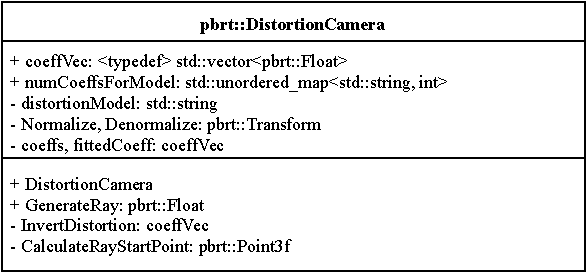
\includegraphics[height=.4\columnwidth]{uml_distortioncam}
	\end{minipage}
	\begin{minipage}{.5\textwidth}
		\centering
		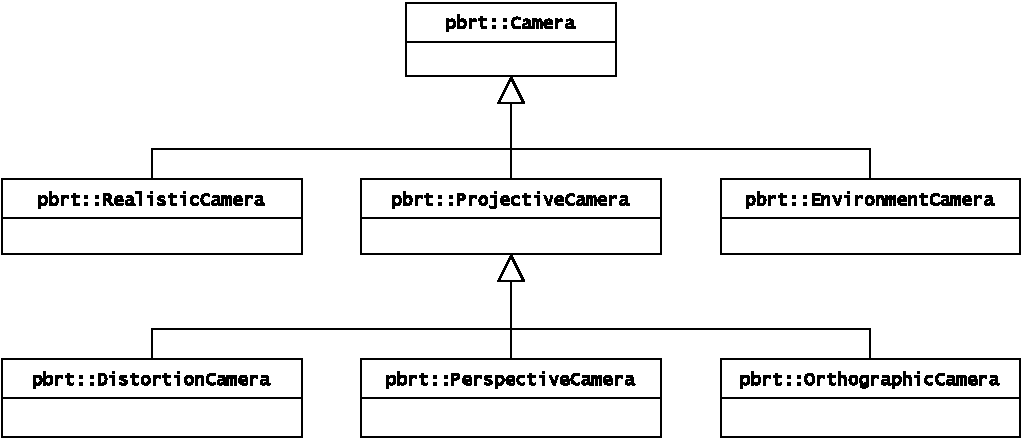
\includegraphics[height=.4\columnwidth]{uml_classes}
	\end{minipage}
	\caption{UML-Darstellung von \texttt{DistortionCamera} (links) und Einordnung in die Klassenstruktur der vorhandenen Kameraklassen (rechts).}
	\label{fig:uml}
\end{figure}


Im Konstruktor der Klasse wird zunächst eine Validierung des übergebenen Verzerrungsmodell durchgeführt. Ist kein Modell in der zu rendernden Szene definiert, so wird die inverse Verzerrungsfunktion zu $f(r) = r$ gesetzt. Das Rendering entspricht dann dem einer \texttt{PerspectiveCamera}. Anschließend wird überprüft, ob das übergebende Modell implementiert ist und die korrekte Anzahl an Koeffizienten übergeben wurde. Dies geschieht anhand der Variablen \texttt{numCoeffsForModel}. Sind die Eingabeparameter korrekt, wird per LS die inverse Verzerrungsfunktion angenähert. Da alle implementierten Modelle Polynome höchstens fünften Grades darstellen, wird zur Näherung ein Polynom fünften Grades verwendet. 
Des Weiteren wird im Konstruktor die Transformation \texttt{Normalize} (siehe \ref{subsubsec:norm_radius} sowie die dazugehörige inverse Transformation \texttt{Denormalize} definiert. Diese setzen die in Abschnitt \ref{subsubsec:norm_radius} beschriebenen Normalisierung der Pixelkoordinaten um.

\begin{lstlisting}[caption={Transformation zur Normalisierung der Pixelkoordinaten}]
/* -------- Define transformations for ray generation --------*/
Float xRes = film->fullResolution.x;
Float yRes = film->fullResolution.y;
Float cornerRadius = sqrt(pow(xRes/2, 2) + pow(yRes/2, 2)) / 2.;
NormalizeToCornerRadius = Scale(1. / cornerRadius, 1. / cornerRadius, 1.);
Denormalize = Inverse(NormalizeToCornerRadius);
\end{lstlisting}


Zum Bestimmen der inversen Verzerrungsfunktion ist in \texttt{distortion.h} die Funktion \texttt{fitPolyCoeffs} implementiert. Diese setzt das Least Squares Verfahren wie in Abschnitt \ref{subsubsec:least} beschrieben um.
Für die Matrizenoperationen wird dabei auf Funktionen aus der Boost-Bibliothek zurückgegriffen. Boost ist eine Sammlung von Open Source C++-Bibliotheken \cite{boost}. In diesem Fall wird die Unterbibliothek \texttt{Boost::numeric::uBLAS} verwendet \cite{ublas}. BLAS steht dabei für "Basic Linear Algebra Subprograms", was Inhalt und Zielsetzung der Bibliothek gut zusammenfasst. Zusätzlich ist eine Funktion \texttt{evalPolynomial} vorhanden, die für einen gegebenen Satz an $m$ Polynomkoeffizienten $a_i$ und einen Wert $x \in R$ die Funktion $y = a_0 + a_1 x + a_2 x^2 + \dots + a_{m-1} x^{m-1}$ berechnet. In \texttt{InvertDistortion} wird die übergebene Verzerrungsfunktion abgetastet und anschließend der Koeffizientenvektor der inversen Funktion genähert.

\begin{lstlisting}[caption={"Abtasten" des Verzerrungsmodells und Invertierung}]
// fill sample vector according to the model used
for (int i = 0; i < sampleSize; i++) {
	x[i] = i / scale;
	y[i] = (*modelFunc)(x[i], coeffs);
}
coeffVec polyCoeffs = fitPolyCoeffs(y, x, polyDegree);
\end{lstlisting}

Die Erzeugung eines Strahls passiert in der Methode \texttt{GenerateRay}. Dort wird für das aktuelle \texttt{CameraSample} die Methode \texttt{CalculateRayStartingPoint} aufgerufen, um den Ausgangspunkt für den zu erzeugenden Strahl zu bestimmen, wie in \ref{subsubsec:anwenden} beschrieben.
Die Funktion \texttt{GenerateRay} unterscheidet sich von ihrem Äquivalent in der Klasse \texttt{PerspectiveCamera} nur durch die folgende Zeile:

\begin{lstlisting} [caption={Anpassung in der Methode \texttt{GenerateRay}}]
Point3f pCamera = RasterToCamera(CalculateRayStartingpoint(sample));
\end{lstlisting}

Neben dieser eigentlichen Implementierung der neuen Kameraklasse waren noch geringe Anpassungen nötig, um die Parameter für \texttt{DistortionCamera} aus einer \texttt{.pbrt}-Datei zu parsen. Diese betrafen die Funktion \texttt{MakeCamera} in \texttt{/src/core/api.cpp}. Außerdem musste die neue Abhängigkeit von der Boost-Bibliothek in \texttt{CMakeLists.txt} eingepflegt werden. Soll in Zukunft ein weiteres Verzerrungsmodell in die Klasse eingebaut werden, so sind folgende Punkte zu erledigen:
\begin{itemize}
	\item Mögliche neue Parameter müssen in der Funktion \texttt{MakeCamera} aus der Szenenbeschreibung geparsed werden und im Konstruktor von \texttt{DistortionCamera} hinzugefügt werden.
	\item Der Name des neuen Modells und die benötigte Anzahl von Koeffizienten müssen in der Variablen \texttt{numCoeffsForModel} hinzugefügt werden.
	\item Die Funktion, die die eigentliche Modellberechnung durchführt, muss implementiert werden. Die aktuellen Modellfunktionen sind in als \texttt{inline} deklarierten Funktionen in \texttt{distortion.h} implementiert worden.
	\item Schließlich muss die Modellfunktion in \texttt{InvertDistortion} ausgewählt werden, wenn das neue Modell übergeben wird.
\end{itemize}

\subsection{Interface in der Szenenbeschreibung}

Die \texttt{DistortionCamera}-Klasse übernimmt alle Argumente von der \texttt{PerspectiveCamera}. Diese sind in \cite{pbrt_file} bereits dokumentiert. Zusätzlich können folgende Argumente übergeben werden:
\begin{table}[h]
	\begin{tabularx}{\textwidth}{l|l|l|X}
		\textbf{Datentyp} & \textbf{Name} & \textbf{Default} & \textbf{Beschreibung} \\ \hline \hline
		String & model & NO\_MODEL & Name des Verzerrungsmodells. Momentan sind verfügbar: "poly3lensfun", \mbox{"poly5lensfun"}, "ptlens".\\
		Float & coefficients & [0, 1] & Koeffizientenvektor für das gegebene Verzerrungsmodell. \\
		Float & centerx & 0.0 & Verschiebung des Bildmittelpunkts in \mbox{x-Richtung} \\
		Float & centery & 0.0 & Verschiebung des Bildmittelpunkts in \mbox{y-Richtung}
	\end{tabularx}
\end{table}
	\clearpage
	\newpage
\section{Verifizierung und Ergebnisse}
\subsection{Planung}
Zur Verifizierung der in C++ implementierten Verzerrung, wurde ein Auswertungsskript in MATLAB erstellt. Die Grundidee der Verifizierung ist, dass für einfache Szenen die Verzerrung des Bildes durch Änderung des verfolgten Lichtstrahls, ungefähr äquivalent mit der Interpolation eines unverzerrten Bildes, gerendert durch die \texttt{PerspectiveCamera} des pbrt, sein sollte.
Dies wird auf zwei Arten überprüft:
\begin{enumerate}
	\item Das durch \texttt{DistortionCamera} gerenderte Bild, wird mit dem gegebenen Polynom \textbf{entzerrt} und mit dem von \texttt{PerspectiveCamera} gerenderten Bild verglichen
	\item Das durch \texttt{PerspectiveCamera} gerenderte Bild wird mit dem gegebenen Polynom \textbf{verzerrt} und mit dem von \texttt{DistortionCamera} gerenderten Bild verglichen
\end{enumerate}

Als Grundlage des Tests wird das in Abbildung \ref{fig:test_img} dargestellte Punkteraster angenommen. 

\begin{figure}[h]
	\centering
	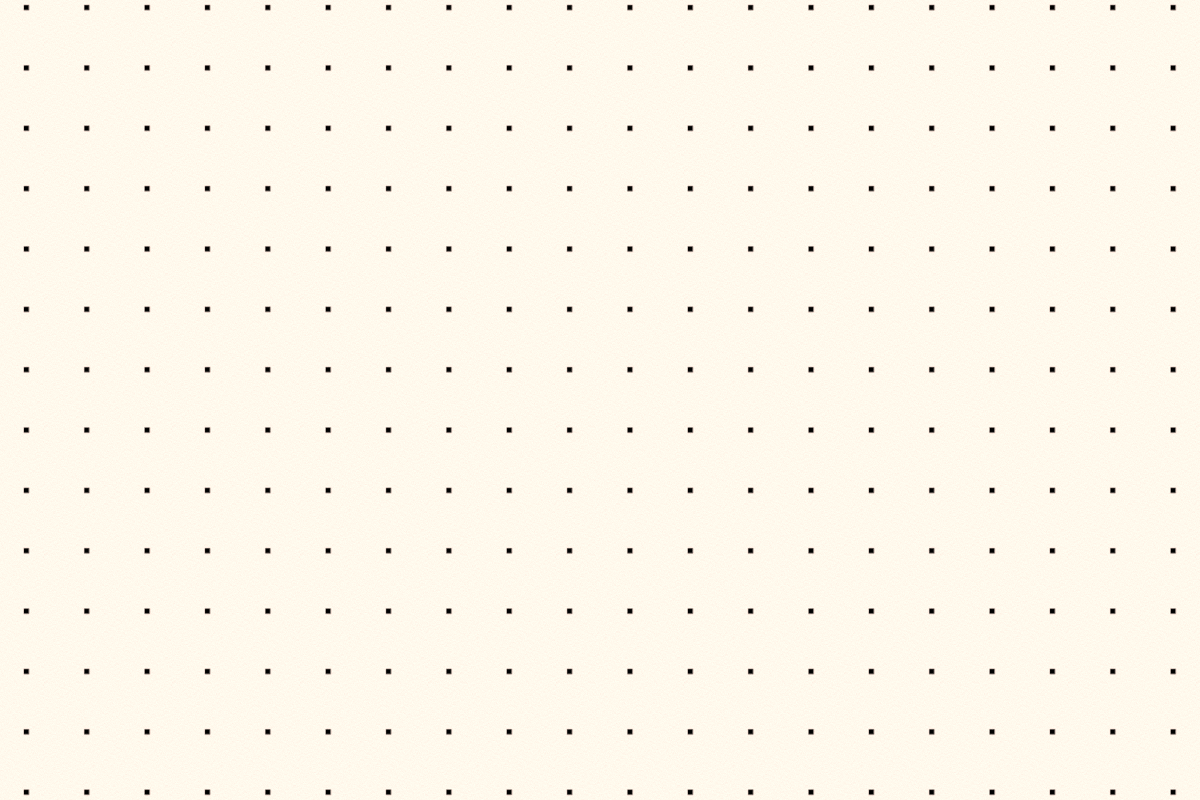
\includegraphics[width=0.5\textwidth]{img/dot_perspective.png}
	\caption{Testbild: Punkteraster, gerendert mit pbrt \texttt{PerspectiveCamera}}
	\label{fig:test_img}
\end{figure}

Es wird zum Einen die Differenz zwischen den Ergebnissen von pbrt und Matlab optisch auf systematische Fehler überprüft, zum Anderen wird die Peak-Signal-to-Noise-Ratio (kurz \textbf{PSNR}) als quantitative Fehlermetrik genutzt.
Diese ergibt sich aus der maximalen Intensität des Bildes $I_\text{max}$ und dem Mean-Square-Error $\text{MSE}$:
\begin{equation}
	PSNR = 10\cdot \log_{10} (I_\text{max}^2/\text{MSE})
\end{equation}

Da die Verzerrung und Entzerrung keine chromatischen Aberrationen mit einbezieht, wird jeder Farbkanal mit der gleichen Verzerrung berechnet. Aus diesem Grund werden zum Vergleich lediglich Grauwerte gezeigt.

\subsection{Implementierung in Matlab}
Die Ver- und Entzerrung in Matlab erfolgt durch eine Funktion namens \texttt{distortImage}. Diese nimmt als Eingangswerte ein Eingangsbild und ein Array von Polynomkoeffizienten sowie mehrere optionale Parameter entgegen. Die optionalen Übergabeparameter erlauben ein Verschieben des Bildmittelpunktes und die Auswahl zwischen Ver- und Entzerrung des Bildes mit den gegebenen Koeffizienten. 

Als erster Schritt werden jedem Bildpunkt die normierten X und Y Koordinaten zugewiesen und in ein Format gebracht, welches der Interpolant entgegen nimmt:
\begin{lstlisting}[style=Matlab-editor,basicstyle=\mlttfamily]
%% Bestimmung der normierten X und Y-Koordinaten mit Center-Offset
xRange = scale*((-(Lx-1)/2:(Lx-1)/2)-cx);
yRange = scale*((-(Ly-1)/2:(Ly-1)/2)-cy);
[X,Y] = meshgrid(yRange,xRange);

\end{lstlisting}

Anschließend werden für jeden Bildpunkt neue Koordinaten nach Verzerrung durch das gegebene Polynom bestimmt:

\begin{lstlisting}[style=Matlab-editor,basicstyle=\mlttfamily]
%% Berechne das Verzerrungspolynom und verzerrte XY Coordinaten
function [distortedX,distortedY] = distortXY(X,Y,polyCoefficients)
  R = sqrt(X.^2+Y.^2);
  R_factor = zeros(size(R));
  for index = 1:numel(polyCoefficients)
    exponent = index-1;
    R_factor = R_factor+polyCoefficients(index)*R.^(exponent);
  end
  distortedX = X.*R_factor;
  distortedY = Y.*R_factor;
end
\end{lstlisting}

Je nach Ver- oder Entzerrung wird von den normierten in die verzerrten Koordinaten interpoliert oder umgekehrt.
\begin{lstlisting}[style=Matlab-editor,basicstyle=\mlttfamily]
%% Berechnung der X,Y Position nach Ver/Entzerrung
if strcmp(mode,'distort')
	img_vector = reshape(img,pixelCount,1);
	P = cat(3,distortedX,distortedY);
	%%
	P = reshape(P,pixelCount,2);
	interpolant = scatteredInterpolant(P,img_vector,'linear','none');
	imgOut = interpolant(X,Y);
elseif strcmp(mode,'undistort')
	imgOut = interpn(X,Y,img,distortedX,distortedY,'linear',NaN);
end
\end{lstlisting}


\subsection{Region-Of-Interest}
\label{sec:roi}
Die Interpolatoren sind so konfiguriert, dass die Bildbereiche außerhalb des gültigen Wertebereiches einen NaN Wert erhalten. Alle Werte, die erfolgreich interpoliert werden, bilden die Region-Of-Interest (kurz \textbf{ROI}) für einen Vergleich der Bilder.
\begin{lstlisting}[style=Matlab-editor,basicstyle=\mlttfamily]
%% Bestimmung der Region of Interest für Entzerrung
roi = ~isnan(imgOut);
\end{lstlisting}
Der für die Verzerrung \texttt{ScatteredInterpolant} interpoliert zwischen gegebenen Bildpunkten auf Basis einer Triangulation der Punkte. Die gesamte Basis interpolierbarer Punkte ist dabei die konvexe Hülle der Gesamtpunkte (vgl. Abbildung~\ref{fig:convex_hull}). Einige dieser Punkte wären bei einer unverzerrten Kamera außerhalb des Bildes, daher kann die Interpolation in diesem Bereich keine sinnvollen Werte liefern. Im Folgenden wird der fehlerhafte Bereich dennoch als Teil der ROI beachtet, da die Bestimmung einer passenden konkaven Hülle den Umfang dieser Arbeit überschreiten würde.
\begin{figure}[h]
	\begin{minipage}{.3\textwidth}
		\centering
		
\includegraphics[width=\textwidth]{img/pc.png}
		\caption{Punktwolke von Bildpunkten}
		\label{fig:pointcloud}
	\end{minipage}
	\begin{minipage}{.3\textwidth}
	\centering
	
\includegraphics[width=\textwidth]{img/distortedpc.png}
	\caption{Punktwolke verzerrter Bildpunkte}
	\label{fig:distorted_pointcloud}
	\end{minipage}
	\begin{minipage}{.3\textwidth}
		\centering
		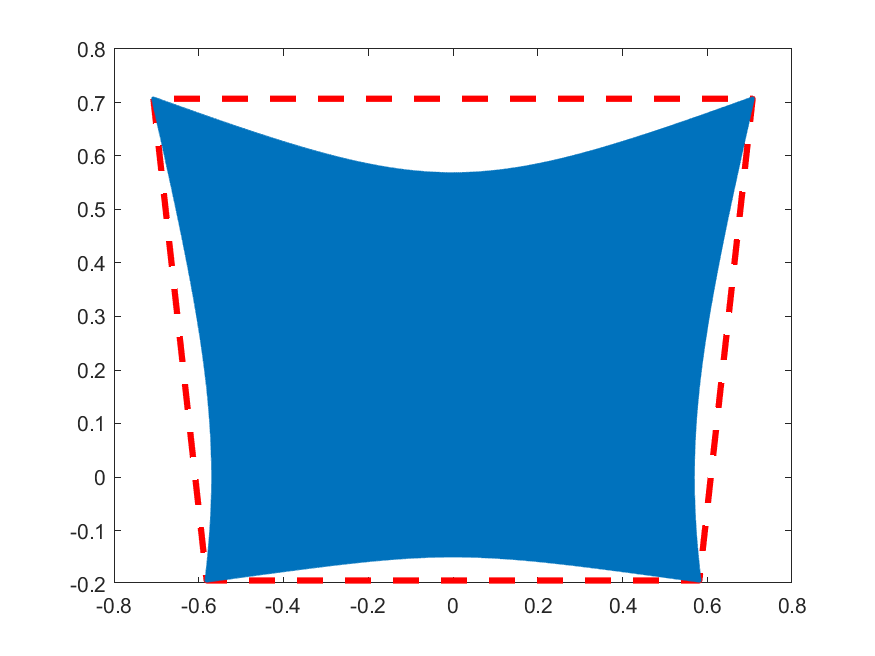
\includegraphics[width=\textwidth]{img/convexpc.png}
		\caption{Konvexe Hülle der verzerrten Bildpunkte}
		\label{fig:convex_hull}
	\end{minipage}
\end{figure}

\subsection{Vergleich}
Die Basis des folgenden Vergleiches bildet eine Reihe von gerenderten Verzerrungen:
\begin{description}
	\item[Verzerrungsmodell] Poly3-Modell
	\item[Bildmittelpunkt-Offset] $X$: $0$, $Y$: $0.5$
	\item[Koeffizient $k_1$] Von $k_1 = 0.0125$ wiederholt verdoppelt bis $k_1 = 0.4$.
\end{description}
Sowohl das Testbild aus Abbildung~\ref{fig:test_img}, die gerenderten Testbilder und die daraus in Matlab entstandenen Bilder sind im dieser Arbeit zugehörigen Git-Repository \cite{git-Distortion_Camera} zu finden. Beispiele sind in Abbildung~\ref{fig:rendered_examples} zu sehen.
\begin{figure}[h]
	\centering
	\begin{minipage}{.3\textwidth}
		\centering
		\includegraphics[width=\textwidth]{img/pbrtDistorted/{dots_poly3_0.0125_cxy_0_0.5}.png}
		\caption*{$0.0125$}
		\label{fig:render_0_0125}
	\end{minipage}
	\begin{minipage}{.3\textwidth}
		\centering
		\includegraphics[width=\textwidth]{img/pbrtDistorted/{dots_poly3_0.1_cxy_0_0.5}.png}
		\caption*{$0.1$}
		\label{fig:render_0_1}
	\end{minipage}
	\begin{minipage}{.3\textwidth}
		\centering
		\includegraphics[width=\textwidth]{img/pbrtDistorted/{dots_poly3_0.4_cxy_0_0.5}.png}
		\caption*{$0.4$}
		\label{fig:render_0_4}
	\end{minipage}
	\caption{Render mit verschiedenen $k_1$ Werten}
	\label{fig:rendered_examples}
\end{figure}

Abbildung~\ref{fig:difference_example} zeigt die Wertedifferenz des perspektivisch gerenderten Bildes und der Entzerrung. Auf diesem Bild, wie auch den restlichen Testbildern ist kein systematischer Unterschied bei der Positionierung der Punkte zu erkennen. 

Es lässt sich vermuten, dass die Fehler an den Kanten lediglich durch die Interpolation entstehen. 

In Abbildung~\ref{fig:difference_dist_0_4} ist im oberen Bildrand zu erkennen, wie Punkte welche durch den pbrt abgebildet werden, durch Matlab nicht korrekt interpoliert werden können. Hier trifft die in Abschnitt~\ref{sec:roi}  beschriebene fehlerhafte Interpolation innerhalb der konvexen Hülle ein. 
\begin{figure}[h]
		\centering
		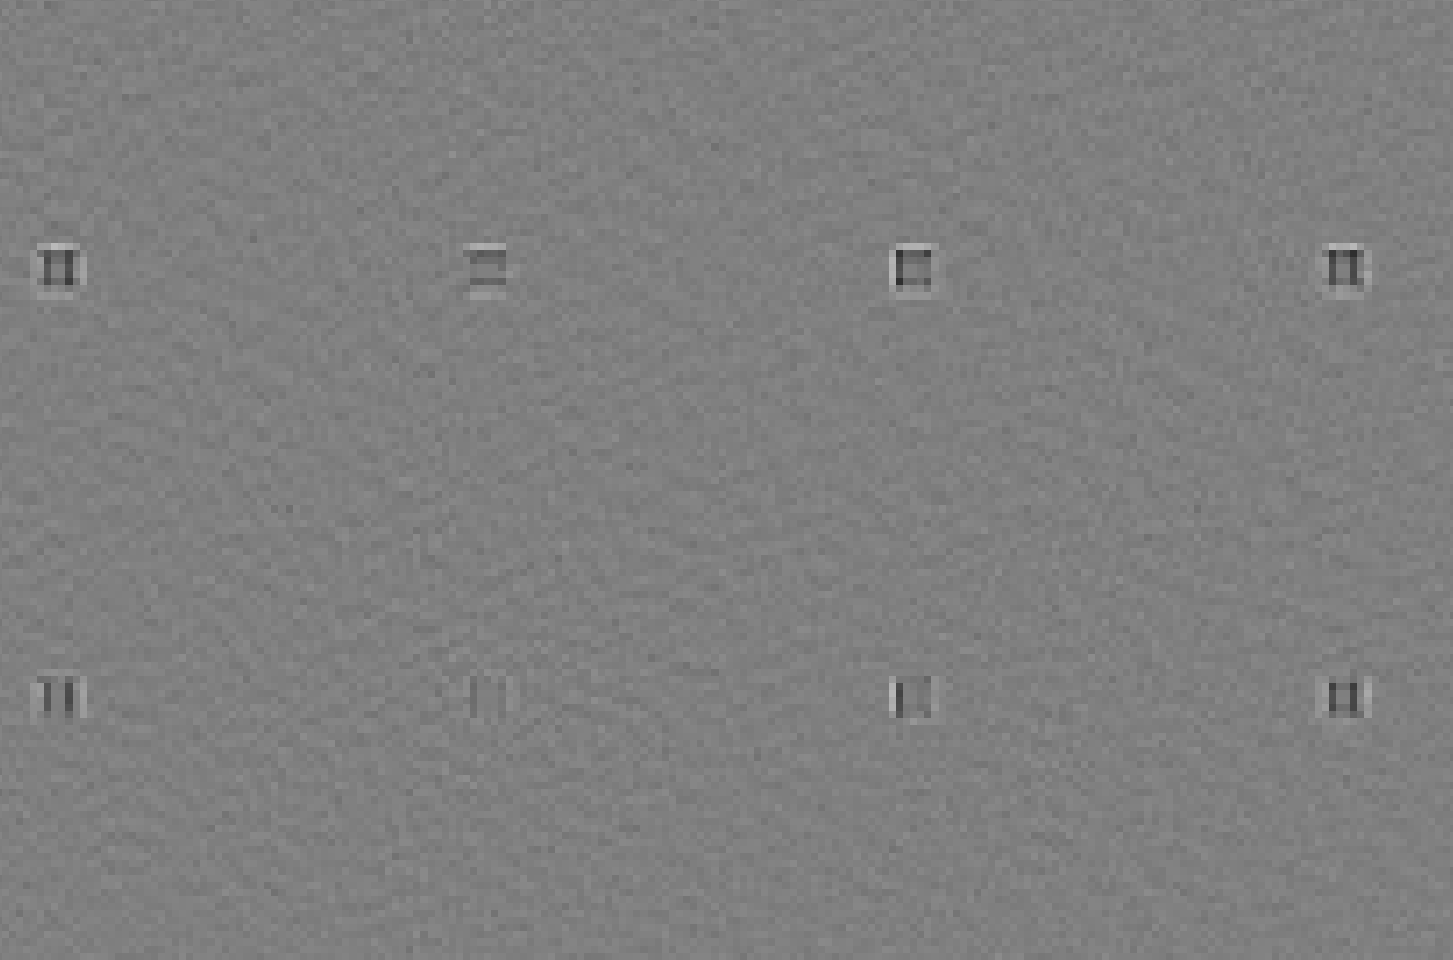
\includegraphics[width=.5\textwidth]{img/error_shape.png}
		\caption{Wertedifferenz zwischen perspektivischem Render und Entzerrung (vergrößert)}
		\label{fig:difference_example}
\end{figure}

\begin{figure}[h]
		\centering
		\begin{minipage}{.49\textwidth}
			\centering
			\includegraphics[width=\textwidth]{img/differenceDistorted/{dots_poly3_0.4_cxy_0_0.5}.png}
			\subcaption{Differenz Matlab- und pbrt-Verzerrung}
			\label{fig:difference_dist_0_4}
		\end{minipage}
		\begin{minipage}{.49\textwidth}
			\centering
			\includegraphics[width=\textwidth]{img/differenceUndistorted/{dots_poly3_0.4_cxy_0_0.5}.png}
			\subcaption{Differenz Matlab-Entzerrung und Test-Bild}
		\end{minipage}
	\caption{Wertedifferenzen von Ent-/Verzerrung mit $k_1 = 0.4$ Mittleres Grau = Kein Fehler, Schwarz/Weiß: Vorzeichenbehafteter Fehler}
	\label{fig:difference_0_4}
\end{figure}

Tabelle~\ref{tbl:comparison} zeigt den Einfluss der stärke der Verzerrung, auf die Ähnlichkeit der Ergebnisse von Matlab und pbrt. Grundsätzlich ergibt sich aus einer stärkeren Verzerrung ein größerer Interpolationsfehler. 

Die PSNR-Werte bei Tests mit anderen Verzerrungsmodellen sind im gleichen Wertebereich (ca. $37-40\text{ dB}$ bei geringer Verzerrung). Bei der Verschiebung des perspektivischen Bildes um einen halben Pixel ergibt sich beim Vergleich mit der unverschobenen Version eine PSNR von $32.22 \text{ dB}$.

Insgesamt kann daher davon ausgegangen werden, dass das entwickelte pbrt Modell die Verzerrung korrekt anwendet.

\begin{table}
	\centering
\begin{tabular}{|c|c|c|c|c|}
	\hline 
	\rule[-1ex]{0pt}{2.5ex}  & \multicolumn{2}{c|}{Entzerrung} & \multicolumn{2}{c|}{Verzerrung}  \\ 
	\hline 
	\rule[-1ex]{0pt}{2.5ex} $k_1$ & $\text{PSNR}/\text{dB}$ & $|e_\text{MAX}|$ & $\text{PSNR}/\text{dB}$ & $|e_\text{MAX}|$ \\ 
	\hline 
	\rule[-1ex]{0pt}{2.5ex} 0.0125 & 40.02 & 0.2366 & 39.90 & 0.2701 \\ 
	\hline 
	\rule[-1ex]{0pt}{2.5ex} 0.025 & 40.00 & 0.2488 & 39.93 & 0.2588 \\ 
	\hline 
	\rule[-1ex]{0pt}{2.5ex} 0.05 & 39.72 & 0.2675 & 39.88 & 0.2918 \\ 
	\hline 
	\rule[-1ex]{0pt}{2.5ex} 0.1 & 39.59 & 0.2667 & 40.08 & 0.2907 \\ 
	\hline 
	\rule[-1ex]{0pt}{2.5ex} 0.2 & 38.86 & 0.3357 & 38.87 & 0.9769 * \\ 
	\hline 
	\rule[-1ex]{0pt}{2.5ex} 0.4 & 35.42 & 0.5514 & 33.16 & 0.9865 * \\ 
	\hline 
\end{tabular} 

\caption{Auswertung der Reihe von Bildern mit PSNR und maximalem Absolutfehler (höchster Bildwert ist 1). Mit * markierte Werte stammen von der ungenauen ROI (Abschnitt~\ref{sec:roi})}
\label{tbl:comparison}
\end{table}










 

	\clearpage
	\newpage
\section{Ergebnisse, Diskussion und Ausblick}

In der durchgeführten Arbeit hat sich gezeigt, dass mit einer relativ kleinen Modifikation eine Implementierung von gemessenen Verzeichnungen realer Objektive in den vorhandenen Source Code von \textit{pbrt} eingefügt werden konnte. Die einzige Schwierigkeit bestand darin, eine Invertierung der gemessenen Verzerrung zu bilden, welche numerisch errechnet werden musste. Anschließend konnten die damit durchgeführten Verzerrungen, wie sie exemplarisch in Abbildung \ref{fig:Guitar} an einem gerenderten Gitarren-Griffbrett zu sehen sind, mit einer bereits vorhandenen Matlab Implementierung verifiziert werden, wobei sich die geringen Unterschiede der beiden Ergebnisse auf Ungenauigkeiten aufgrund von Interpolation zurückführen lassen.\\


\begin{figure}[h]
	\begin{subfigure}{.5\textwidth}
		\raggedleft
		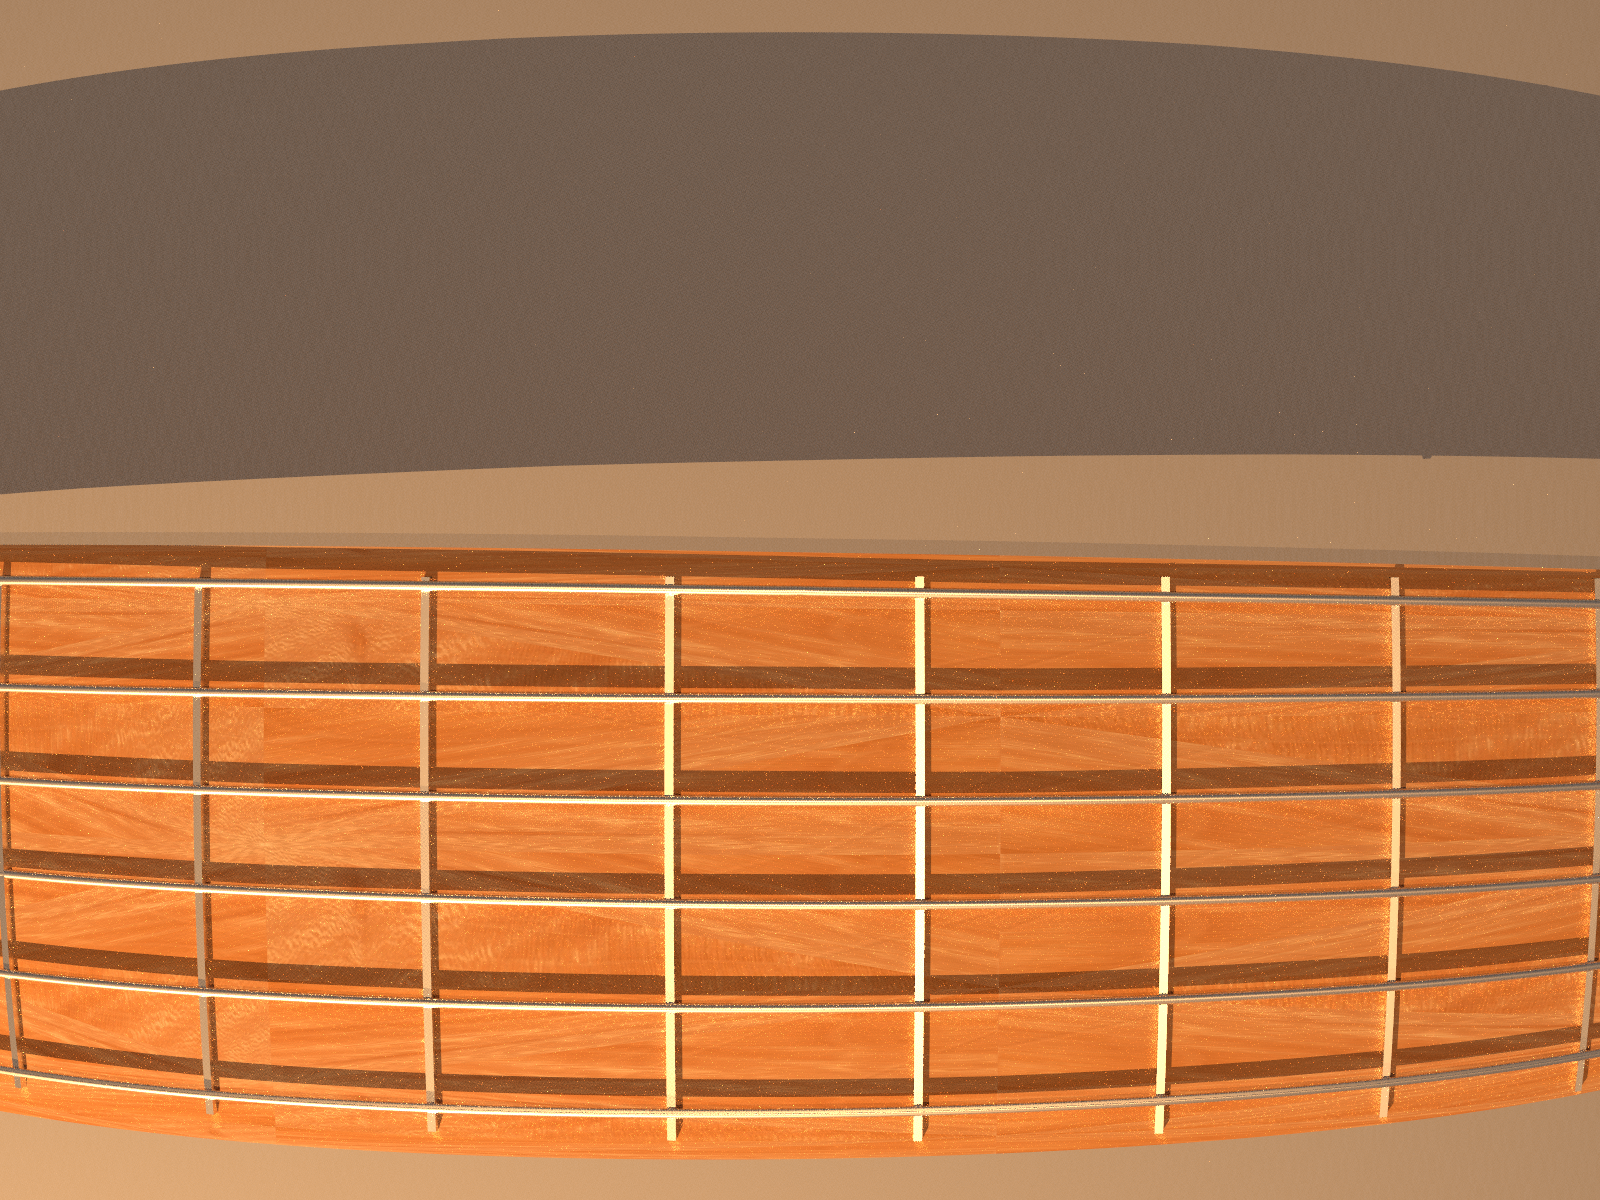
\includegraphics[width=\textwidth]{img/guitarDistorted.png}
		\caption{Poly3-Modell und $k=0.2$}
	\end{subfigure}
\begin{subfigure}{.5\textwidth}
		\raggedright
		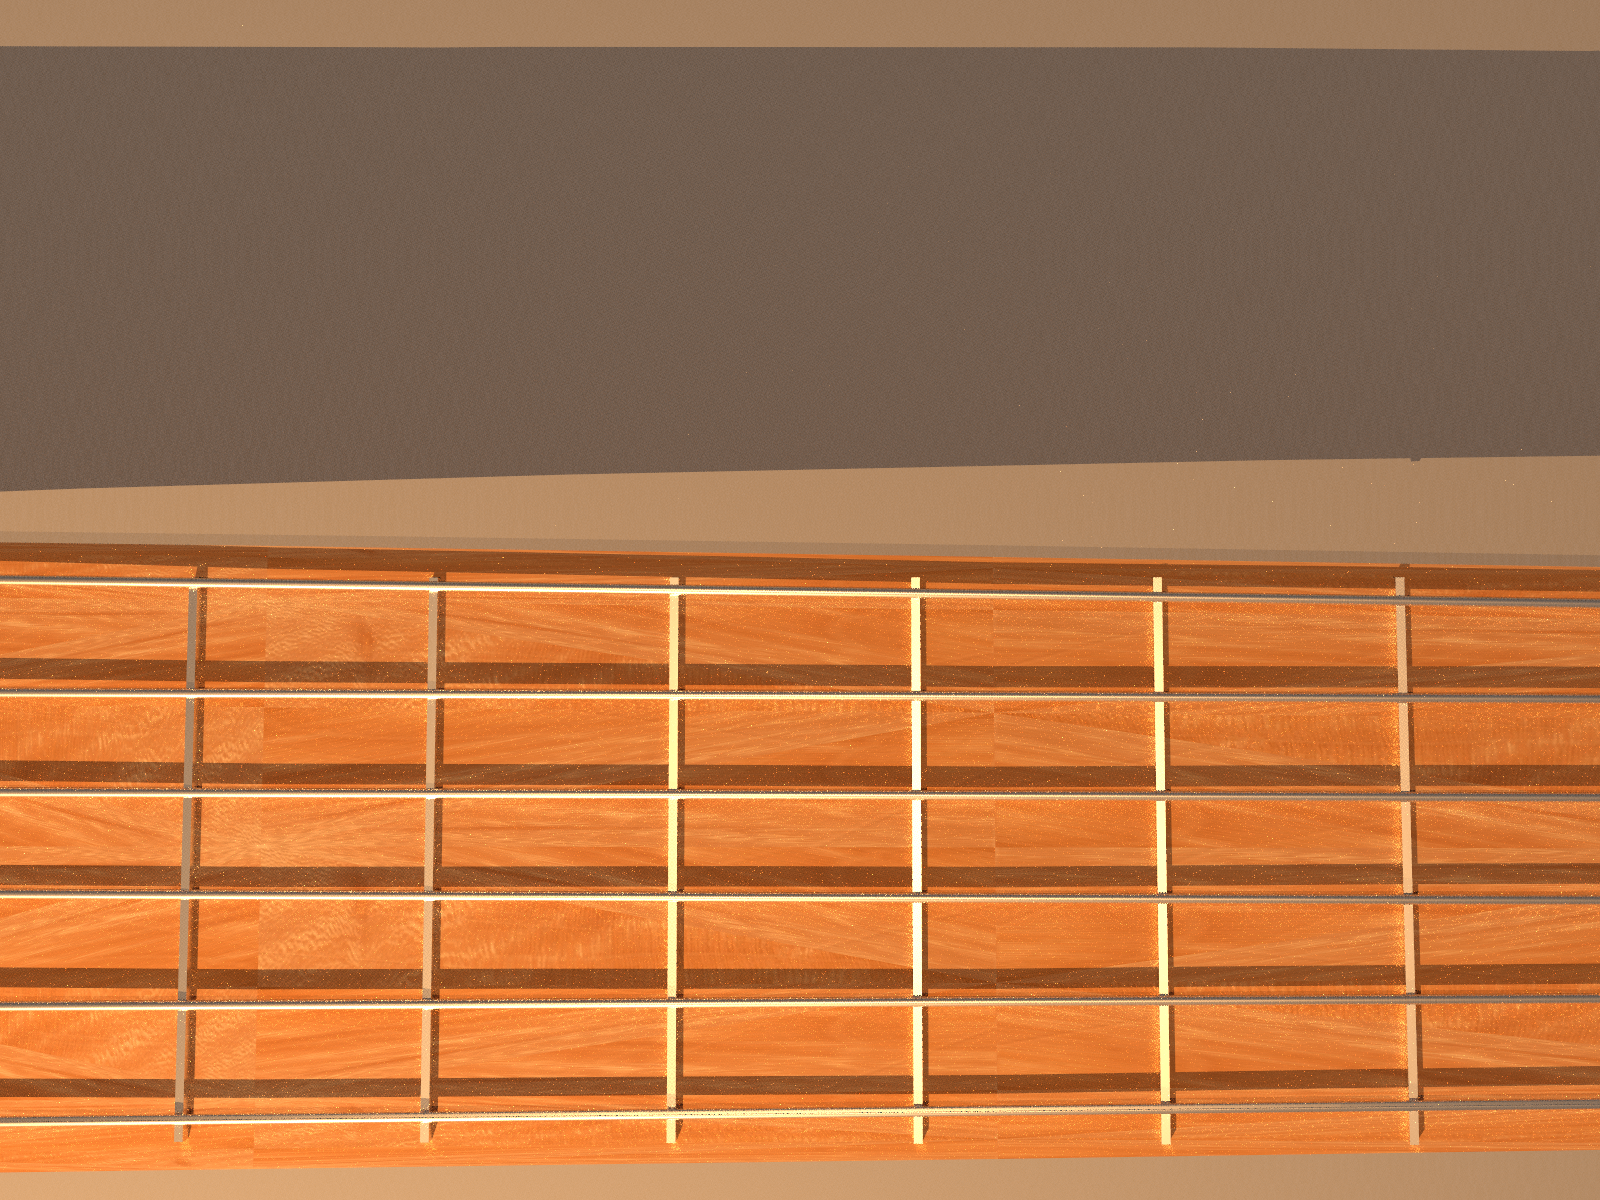
\includegraphics[width=\textwidth, ]{img/guitarUndist.png}
		\caption{Unverzerrt mit perspectiv camera}
	\end{subfigure}
\caption{Gerendertes Gitarrengriffbrett}
\label{fig:Guitar}
\end{figure}


Mögliche Erweiterungen der hier durchgeführten Implementierung könnten eine Verzerrung nach einem nicht radialsymmetrischen Modell umfassen. Auch wenn sich die meisten Verzeichnungen von Objektiven mit den hier genutzten Modellen gut abbilden lassen, liegt in der Realität nicht unbedingt eine komplett radialsymmetrische Verzerrung vor. So kann eine größere Genauigkeit durch ein getrenntes Abbilden der Verzerrung für x- und y-Richtung oder Hinzufügen einer Tangentialkomponente zur Radialverzerrung erreicht werden. Auch das momentan in der Alpha Version von Lensfun integrierte Verzerrungsmodell nach Adobe Vorgaben kann integriert werden, wenn dessen Implementierung ausreichend getestet ist. Desweiteren wäre denkbar, die Übergabe von gemessenen Verzerrungen nicht nur durch Modellparameter zu erlauben, sondern direkt als Matrix gemessener Abweichungen für bestimmte Pixelkoordinaten. Aus diesen Daten könnte dann ohne den Umweg über das "Abtasten" der Modellfunktion direkt eine inverse Verzerrungsfunktion bestimmt werden.
Als weiteren Ausblick kann außerdem die Implementierung von Randabdunklungseffekten (Vignettierung) gesehen werden, um eine weitere in der Realität auftretende Eigenschaft von Optiken zu berücksichtigen. 
	\clearpage
	\bibliographystyle{plain}
	\bibliography{quellen}
	
\end{document}
